\graphicspath{{figures/appendix/}}
\chapter{Test Journal: Gear Train System}\label{appendix:DCMotorInductance}
\begin{table}[htbp]
\begin{tabular}{l l}
\textbf{Test participants:} & Maxime \& Geoffroy  \\
\textbf{Date:}  & 28/2/2017
\end{tabular}
\end{table}

\section*{Purpose}
The objective of this test is to determine all the of the gear train system composed of the DC motor and the gear train.
\section*{Electronics characteristics}

\subsection*{Internal Resistance and Inductance of the DC Motor $R_m$, $L_m$}
\subsection{Internal Resistance of the DC Motor $R_m$}\label{sec:MeasRm}
\begin{table}[htbp]
	\centering
	\caption{List of measurement equipment and components}\label{tab_appendix:RMSetUp}
	
	\begin{tabularx}{\textwidth}{lXXXX}
		Name 				& Brand	& Model & AAU-number									\\ \toprule \rowcolor{lightGrey}
		Oscilloscope	& Agilent & 54621D & 33941 	\\
		Powersupply	& Agilent & E3631A & 78577\\ \rowcolor{lightGrey}
		DC motor & Alsthom BBC & F9M2& 08339
	\end{tabularx}
\end{table}


The first parameter to be tested is the internal resistance of the motor $R_m$. This resistance is needed in the motor's transfer function and will be used to determine the other parameters of the motor. 
\subsubsection*{Setup}
\autoref{fig:RmMeasurementSetup} shows a diagram and photo of the measurement set up
\begin{figure}[htbp]
	\centering
	\begin{subfigure}{0.50\textwidth}
		\includegraphics[width=1\textwidth]{figures/appendix/Motor&GearTests/RmTestSetUpDiagram}
		\caption{Diagram of the setup.} \label{fig:RmMeasurementDiagram}
	\end{subfigure}
	\begin{subfigure}{0.40\textwidth}
			\includegraphics[width=\textwidth]{figures/appendix/Motor&GearTests/KtTestPic}
		\caption{Picture of the setup.} \label{fig:RmMeasurementPictures}
	\end{subfigure}
	\caption{The measurement setup.} \label{fig:RmMeasurementSetup}   
\end{figure} 

\subsubsection*{Method}
This test consists of having the motor shaft locked while the voltage is increased by 0.5 V between each measurements.

\subsubsection*{Raw data}
\autoref{tab_appendix:RmData} is the plotted evolution of the voltage of the circuit according to the current.

\begin{table}[htbp]
	\centering
	\caption{Raw data used to determine $R_m$}\label{tab_appendix:RmData}
	\begin{tabularx}{0.35\textwidth}{XX}
		Voltage (V) & Current (A)\\ \toprule \rowcolor{lightGrey}
		0.50 & 0.33 \\
		1.00 & 0.71 \\ \rowcolor{lightGrey}
		1.50 & 1.13 \\
		2.00 & 1.67 \\ \rowcolor{lightGrey}
		2.49 & 2.34 \\
		2.98 & 2.94 \\ \rowcolor{lightGrey}
		3.50 & 3.75 \\
		3.99 & 4.68 \\ \rowcolor{lightGrey}
		4.50 & 5.54 \\
		4.98 & 6.11 \\ \rowcolor{lightGrey}
		5.54 & 6.46 \\
		6.02 & 7.40 \\ \rowcolor{lightGrey}
		6.51 & 8.26 \\
		7.01 & 9.14 
	\end{tabularx}
\end{table}

\subsubsection{Data Processing}
In order to find the motor's resistance $R_m$, the electrical equations of the motor will be used:
\begin{equation}
	U_m = R_m \cdot i + L_m \frac{di}{dt} + K_e\omega_m
\end{equation}

With the motor shaft locked, $\omega_m = 0$. Moreover, the measurements are made a couple seconds after the change in voltage is made. The current is then constant, canceling its derivative. 

The resulting equation is Ohm's law:
\begin{equation}
U_m = R_m \cdot i
\end{equation}


The measurement of voltage according to the current is presented in \autoref{fig:Rmplot}.
\begin{figure}[htbp]
	\includegraphics[width=1\textwidth]{figures/appendix/Motor&GearTests/plotRm}
	\caption{Measurement of voltage according to the current} \label{fig:Rmplot}
\end{figure}

$R_m$ is the slope of the linear approximation (in dashed yellow) of the voltage over the current: 
\begin{subequations} \label{eq:LaEq}
	\begin{flalign}
		&U_m = R_m \cdot i \\
		&R_m \approx \SI{0.82}{\ohm}
	\end{flalign}
\end{subequations}

\newpage
\subsection{Internal Inductance of the DC Motor $L_m$}
\begin{table}[htbp]
	\centering
	\caption{List of measurement equipment and components}\label{tab_appendix:LaSetUp}

	\begin{tabularx}{\textwidth}{lXXXX}
		Name 				& Brand	& Model & AAU-number									\\ \toprule \rowcolor{lightGrey}
		Oscilloscope	& Agilent & 54621D & 33941 	\\
		Powersupply	& Agilent & E3631A & 78577\\ \rowcolor{lightGrey}
		DC motor & Alsthom BBC & F9M2& 08339 
	\end{tabularx}
\end{table}
\subsubsection*{Setup}
\autoref{fig:LaMeasurementSetup} shows a diagram and photo of the measurement set up.
\begin{figure}[htbp]
	\centering
	\begin{subfigure}{0.50\textwidth}
		\includegraphics[width=0.7\textwidth]{figures/appendix/Motor&GearTests/LmDiagram}
		\caption{Diagram of the setup.} \label{fig:LaMeasurementDiagram}
	\end{subfigure}
	\begin{subfigure}{0.40\textwidth}
		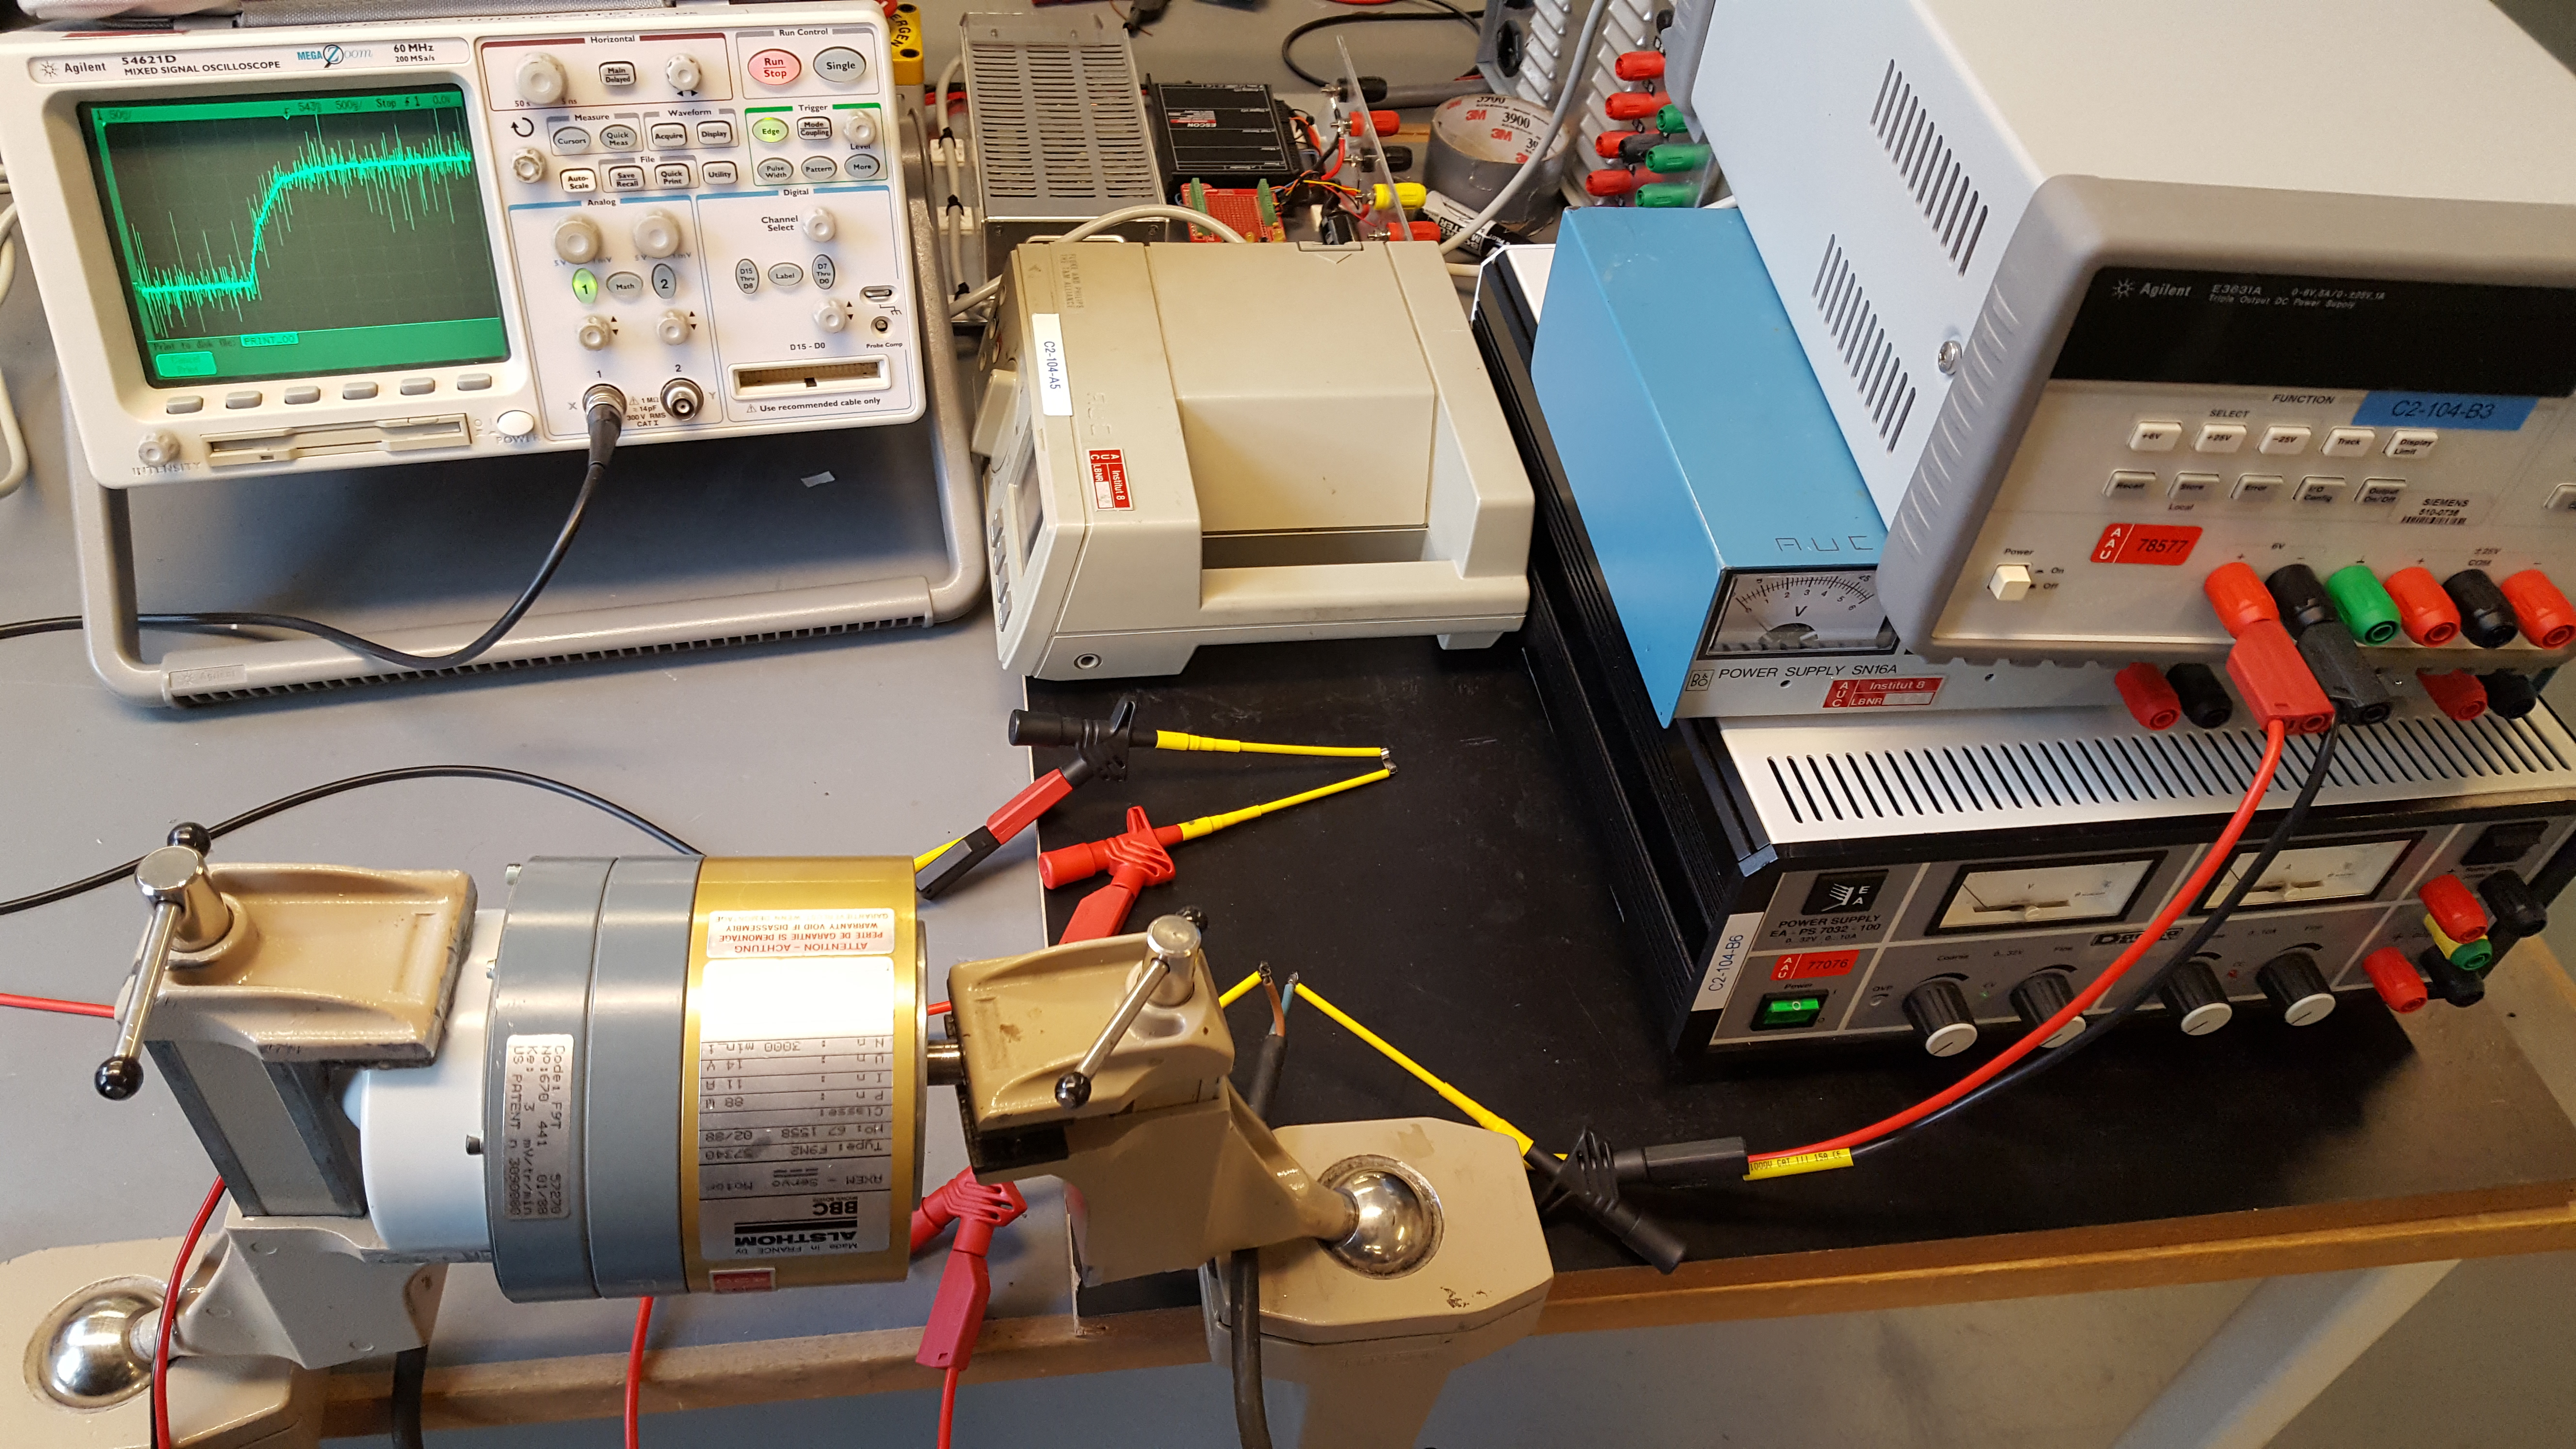
\includegraphics[width=1\textwidth]{MotorImpedanceTest.jpg}
		\caption{Picture of the setup.} \label{fig:LaMeasurementPictures}
	\end{subfigure}
	\caption{$L_m$ measurement setup.} \label{fig:LaMeasurementSetup}   
\end{figure}

\subsubsection*{Method}
This test consists of having the motor shaft locked while a step is applied. The current is measured through the circuit. With the current step response, the inductance of the motor can be found. 
\subsubsection*{Raw data}
\autoref{fig:LaTestCurrentPlot} is the plotted evolution of the current of the circuit in respect to time.

\begin{figure}[htbp]
	\centering
	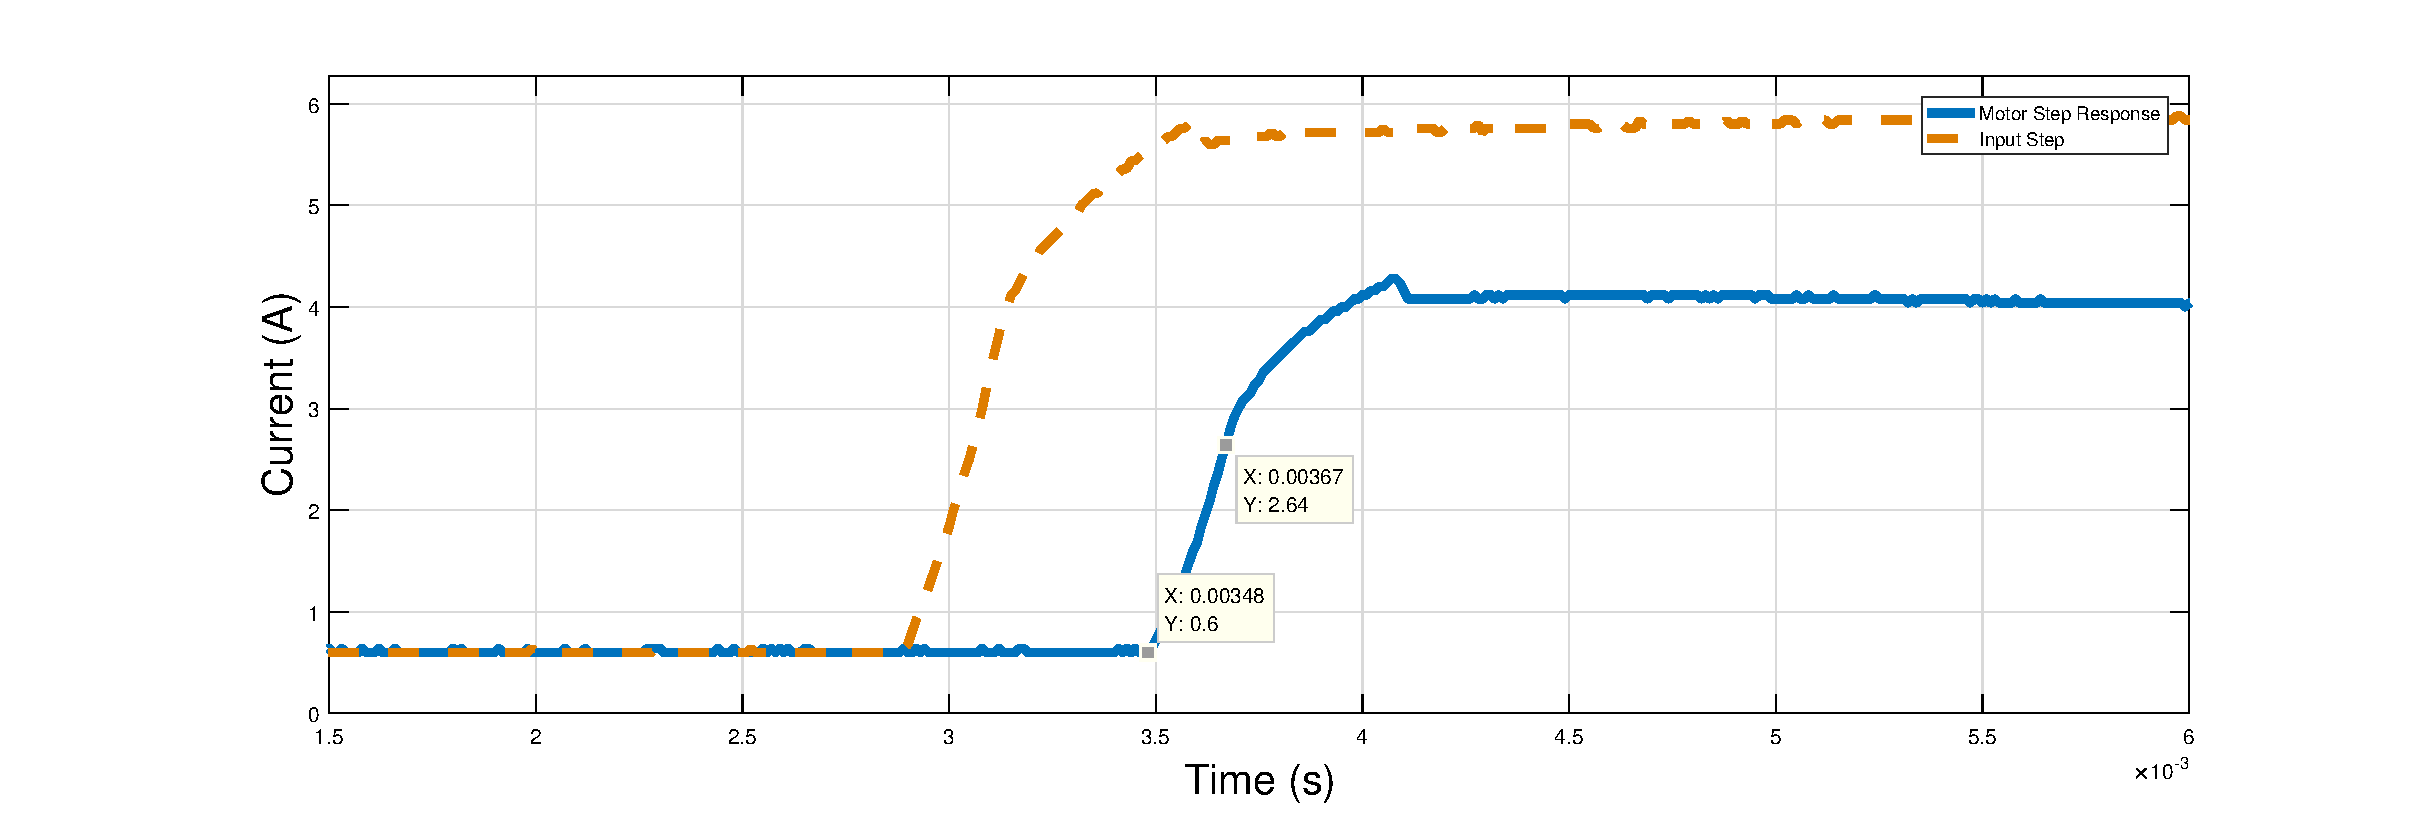
\includegraphics[width=1.2\textwidth]{figures/appendix/Motor&GearTests/PlotLm}
	\caption{Plot of the current step response in respect to time}\label{fig:LaTestCurrentPlot}
\end{figure}

\newpage
\subsubsection*{Data processing}
When the shaft is locked and a step is applied the DC motor's electric equation can be resumed as in \autoref{eq:LmEquation}.
\begin{equation}
	F(s)=\frac{I(s)}{U(s)}=\frac{\frac{1}{R_m}}{\frac{L_m}{R_m} s+1} \addunit{1}
	\label{eq:LmEquation}
\end{equation}
\startexplain
\explain{$I(s)$ is the current in Laplace domain}{1}
\explain{$U(s)$ is the body's acceleration}{1}
\explain{$R_m$ is the internal resistance of the motor}{\si{\ohm}}
\explain{$L_m$ is the internal inductance of the motor}{\si{\henry}}
\stopexplain

When a unit step response is applied to the system \autoref{eq:LmEquation} becomes \autoref{eq:LmEquationStep}.

\begin{equation}
F(s)=\frac{\frac{1}{R_m}}{\frac{L_m}{R_m} s+1}\frac{1}{s}=\frac{-\frac{1}{R_m}}{s+\frac{R_m}{L_m}}+\frac{1}{R_m s} \addunit{1}
\label{eq:LmEquationStep}
\end{equation}

\autoref{eq:LmEquationStep} is then put in the continuous time domain to get \autoref{eq:LmEquationStepTime}.

\begin{equation}
f(t)= \frac{1}{R_m} \left(1-e^{-\frac{R_m}{L_m} t}\right) \addunit{1}
\label{eq:LmEquationStepTime}
\end{equation}

\autoref{eq:LmEquationStepTime} means that at $t=\frac{L_m}{R_m}$ the function would give $1-e^{-1} \approx \SI{63.2}{\percent}$ of its settling value given that the step starts at 0 seconds. Therefore, at \SI{63.2}{\percent} of the settling value $t=\frac{L_m}{R_m}$. \\
Since $R_m=\SI{0.82}{\ohm}$ is known, finding $L_m$ becomes trivial. Here, the step starts at 0.00348 s.

\subsubsection*{Conclusion}

Since the settling value of the output current is \SI{4.04}{\ampere}. Then \autoref{eq:LmEq} gives the value of $L_m$.

\begin{subequations} \label{eq:LmEq}
	\begin{flalign}
		&\frac{1}{R_m} \left(1-e^{-\frac{R_m}{L_m} t}\right) = 4.04 \cdot 0.63212055882 \addunit{\second} \\
		&t \approx 0.00367 - 0.00348 \approx \SI{0.00019}{\second} \\
		&L_m=tR_m \\
		&L_m \approx \SI{156}{\micro\henry}
	\end{flalign}
\end{subequations}


\subsection{The DC Motor velocity constant $K_e$}
\begin{table}[htbp]
	\centering
	\caption{List of measurement equipment and components}\label{tab_appendix:KeSetUp}
	
	\begin{tabularx}{\textwidth}{lXXXX}
		Name 				& Brand	& Model & AAU-number									\\ \toprule \rowcolor{lightGrey}
		Oscilloscope	& Agilent & 54621D & 33941 	\\
		Powersupply	& Agilent & E3631A & 78577\\ \rowcolor{lightGrey}
		DC motor & Alsthom BBC & F9M2& 08339
	\end{tabularx}
\end{table}

\subsubsection*{Setup}
\autoref{fig:KeMeasurementSetup} shows a diagram and photo of the measurement set up
\begin{figure}[htbp]
	\centering
	\begin{subfigure}{0.50\textwidth}
		%\includegraphics[width=0.5\textwidth]{}
		\missingfigure{Diagram of the setup}
		\caption{Diagram of the setup.} \label{fig:KeMeasurementDiagram}
	\end{subfigure}
	\begin{subfigure}{0.40\textwidth}
		%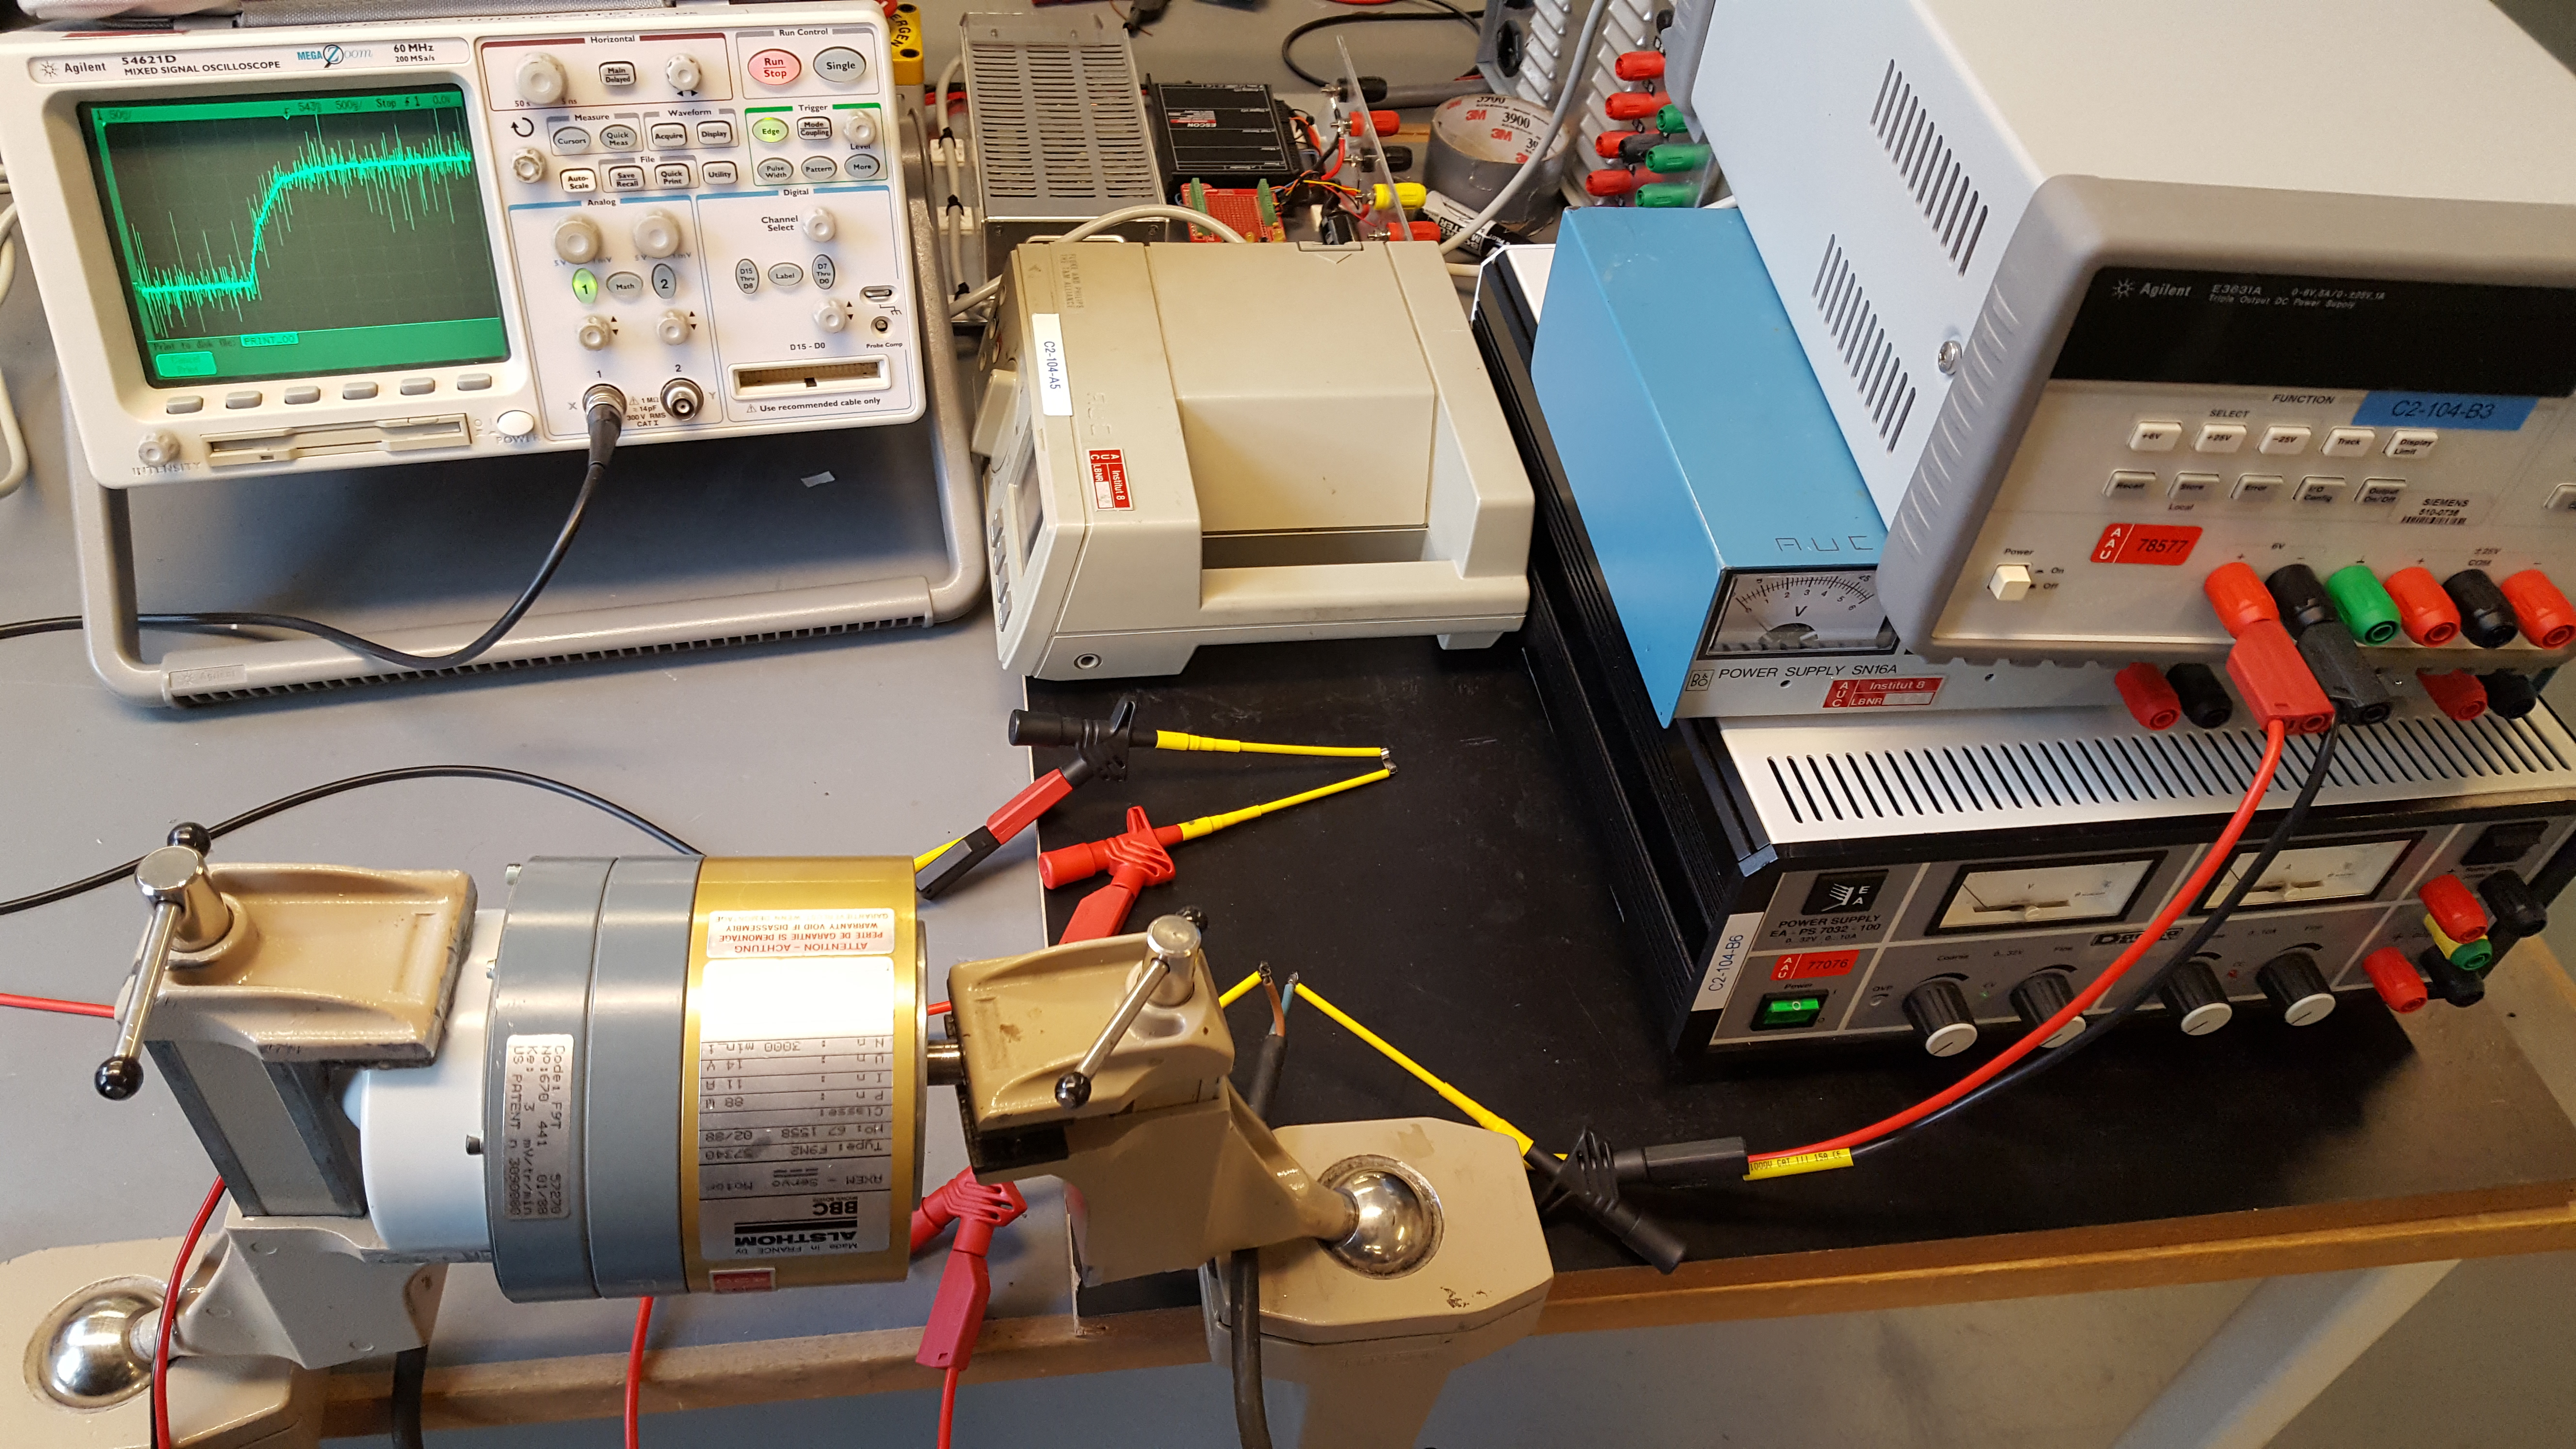
\includegraphics[width=1\textwidth]{MotorImpedanceTest.jpg}
		\missingfigure{Picture of the setup}
		\caption{Picture of the setup.} \label{fig:KeMeasurementPictures}
	\end{subfigure}
	\caption{The measurement setup.} \label{fig:KeMeasurementSetup}   
\end{figure}

\subsubsection*{Method}
This test consists of having the motor shaft rotating in steady state while the voltage $U$ of the generator, the angular velocity $\omega$ of the shaft and the current $I$ are measured.

\subsubsection*{Raw data}
\autoref{tab:KeTest} has all the measurements done.


\subsubsection*{Data processing}

When the shaft is rotating in steady state as shown in \autoref{fig:KeMeasurementDiagram}, \autoref{eq:KeSetUpElec} can be derived.
\begin{equation}
U=K_e\omega+R_m I \addunit{\volt}
\label{eq:KeSetUpElec}
\end{equation}
\startexplain
\explain{$I$ is the current in the circuit}{\si{\ampere}}
\explain{$U$ is the generator's voltage}{\si{\volt}}
\explain{$K_e$ is the velocity constant of the motor}{\si{\volt\per\radian\second}}
\explain{$R_m$ is the internal resistance of the motor}{\si{\ohm}}
\stopexplain

From \autoref{eq:KeSetUpElec} \autoref{eq:KeForm} is obtained by isolating $K_e$.

\begin{equation}
K_e=\frac{U-R_m I}{\omega} \addunit{\volt\per\radian\second}
\label{eq:KeForm}
\end{equation}

\subsubsection*{Conclusion}

\autoref{fig:KeTest} plot the $K_e$ found for each measurement. The $K_e$ used in the model is average of these points. This gives $K_e=\SI{}{\volt\per\radian\second}$

\begin{figure}[htbp]
	\centering
	\includegraphics[width=\textwidth]{RmLmDataPlot}
	\caption{Plot of $K_e$ found for each measures}\label{fig:KeTest}
\end{figure}


\subsection{The DC Motor torque constant $K_t$}
\begin{table}[htbp]
	\centering
	\caption{List of measurement equipment and components}\label{tab_appendix:KtSetUp}
	
	\begin{tabularx}{\textwidth}{lXXXX}
		Name 				& Brand	& Model & AAU-number									\\ \toprule \rowcolor{lightGrey}
		Oscilloscope	& Agilent & 54621D & 33941 	\\
		Powersupply	& Agilent & E3631A & 78577\\ \rowcolor{lightGrey}
		DC motor & Alsthom BBC & F9M2& 08339
	\end{tabularx}
\end{table}

\subsubsection*{Setup}
\autoref{fig:KtMeasurementSetup} shows a diagram and photo of the measurement set up
\begin{figure}[htbp]
	\centering
	\begin{subfigure}{0.50\textwidth}
			\includegraphics[width=\textwidth]{KtTestSetUp}
		\caption{Diagram of the setup.} \label{fig:KtMeasurementDiagram}
	\end{subfigure}
	\begin{subfigure}{0.40\textwidth}
		\includegraphics[width=1\textwidth]{figures/appendix/Motor&GearTests/KtTestPic}
		\caption{Picture of the setup.} \label{fig:KtMeasurementPictures}
	\end{subfigure}
	\caption{The measurement setup.} \label{fig:KtMeasurementSetup}   
\end{figure}

\subsubsection*{Method}
This test consists of having the motor shaft locked while the torque $\tau_m$ and the current $I$ are measured.


\subsubsection*{Raw data}
\autoref{tab_appendix:KtData} has all the measurements done.

\begin{figure}[htbp]
	\centering
	\caption{Raw data used to determine $K_t$}\label{tab_appendix:KtData}
	\begin{tabularx}{0.35\textwidth}{XX}
		Current (A) & $\tau_m$\\ \toprule \rowcolor{lightGrey}
	4.0 & 0.1164 \\
	4.5 & 0.1314 \\ \rowcolor{lightGrey}
	5.0 & 0.1498 \\
	5.5 & 0.1606 \\ \rowcolor{lightGrey}
	6.0 & 0.1824 \\
	6.5 & 0.1896 \\ \rowcolor{lightGrey}
	7.0 & 0.2050 \\
	7.5 & 0.2192 \\ \rowcolor{lightGrey}
	8.0 & 0.2332 \\
	8.5 & 0.2478 \\ \rowcolor{lightGrey}
	9.0 & 0.2604 \\
	9.5 & 0.2750 \\ \rowcolor{lightGrey}
	10.0 & 0.2900
	\end{tabularx}
\end{figure}

\subsubsection*{Data processing}

When the motor is in steady state and the shaft locked as shown in \autoref{fig:KtMeasurementDiagram}, \autoref{eq:KtTest} is found from \autoref{eq:MotorTorque}.

\begin{equation}\label{eq:KtTest}
	K_t=\frac{\tau_m}{I} \addunit{\newton\meter\per\ampere}
\end{equation}

\startexplain
\explain{$I$ is the current in the circuit}{\si{\ampere}}
\explain{$\tau_m$ is the torque of the motor}{\si{\newton\meter}}
\explain{$K_t$ is the motor's torque constant}{\si{\newton\meter\per\ampere}}
\stopexplain

\subsubsection*{Conclusion}

\autoref{fig:KtTest} plot the $K_t$ found for each measurement. The $K_t$ used in the model is average of these points. This gives $K_t=\SI{0.0293}{\newton\meter\per\ampere}$

\begin{figure}[htbp]
	\centering
	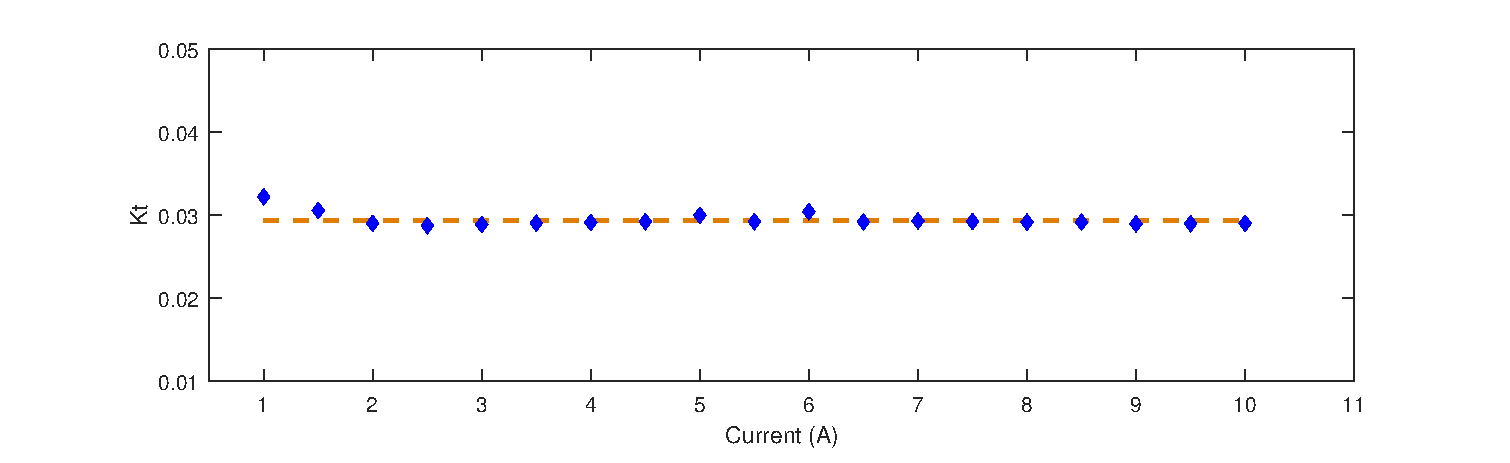
\includegraphics[width=\textwidth]{figures/appendix/Motor&GearTests/PlotKt}
	\caption{Plot of $K_t$ found for each measures}\label{fig:KtTest}
\end{figure}
	

It should be noticed that $K_e$ and $K_t$ values are close, which comforts the results of the tests since they are theoretically equal.

\section{Mechanical Characteristics}

\subsection{Frictions $B_m$}
\begin{table}[htbp]
	\centering
	\caption{List of measurement equipment and components}\label{tab_appendix:BmSetUp}
	
	\begin{tabularx}{\textwidth}{lXXXX}
		Name 				& Brand	& Model & AAU-number									\\ \toprule \rowcolor{lightGrey}
		Oscilloscope	& Agilent & 54621D & 33941 	\\
		Powersupply	& Agilent & E3631A & 78577\\ \rowcolor{lightGrey}
		DC motor & Alsthom BBC & F9M2& 08339
	\end{tabularx}
\end{table}

\subsubsection*{Setup}
\autoref{fig:BmMeasurementSetup} shows a diagram and photo of the measurement set up
\begin{figure}[htbp]
	\centering
	\begin{subfigure}{0.50\textwidth}
		\includegraphics[width=\textwidth]{BmTestSetUp}
		\caption{Diagram of the set up.} \label{fig:BmMeasurementDiagram}
	\end{subfigure}
	\begin{subfigure}{0.40\textwidth}
		%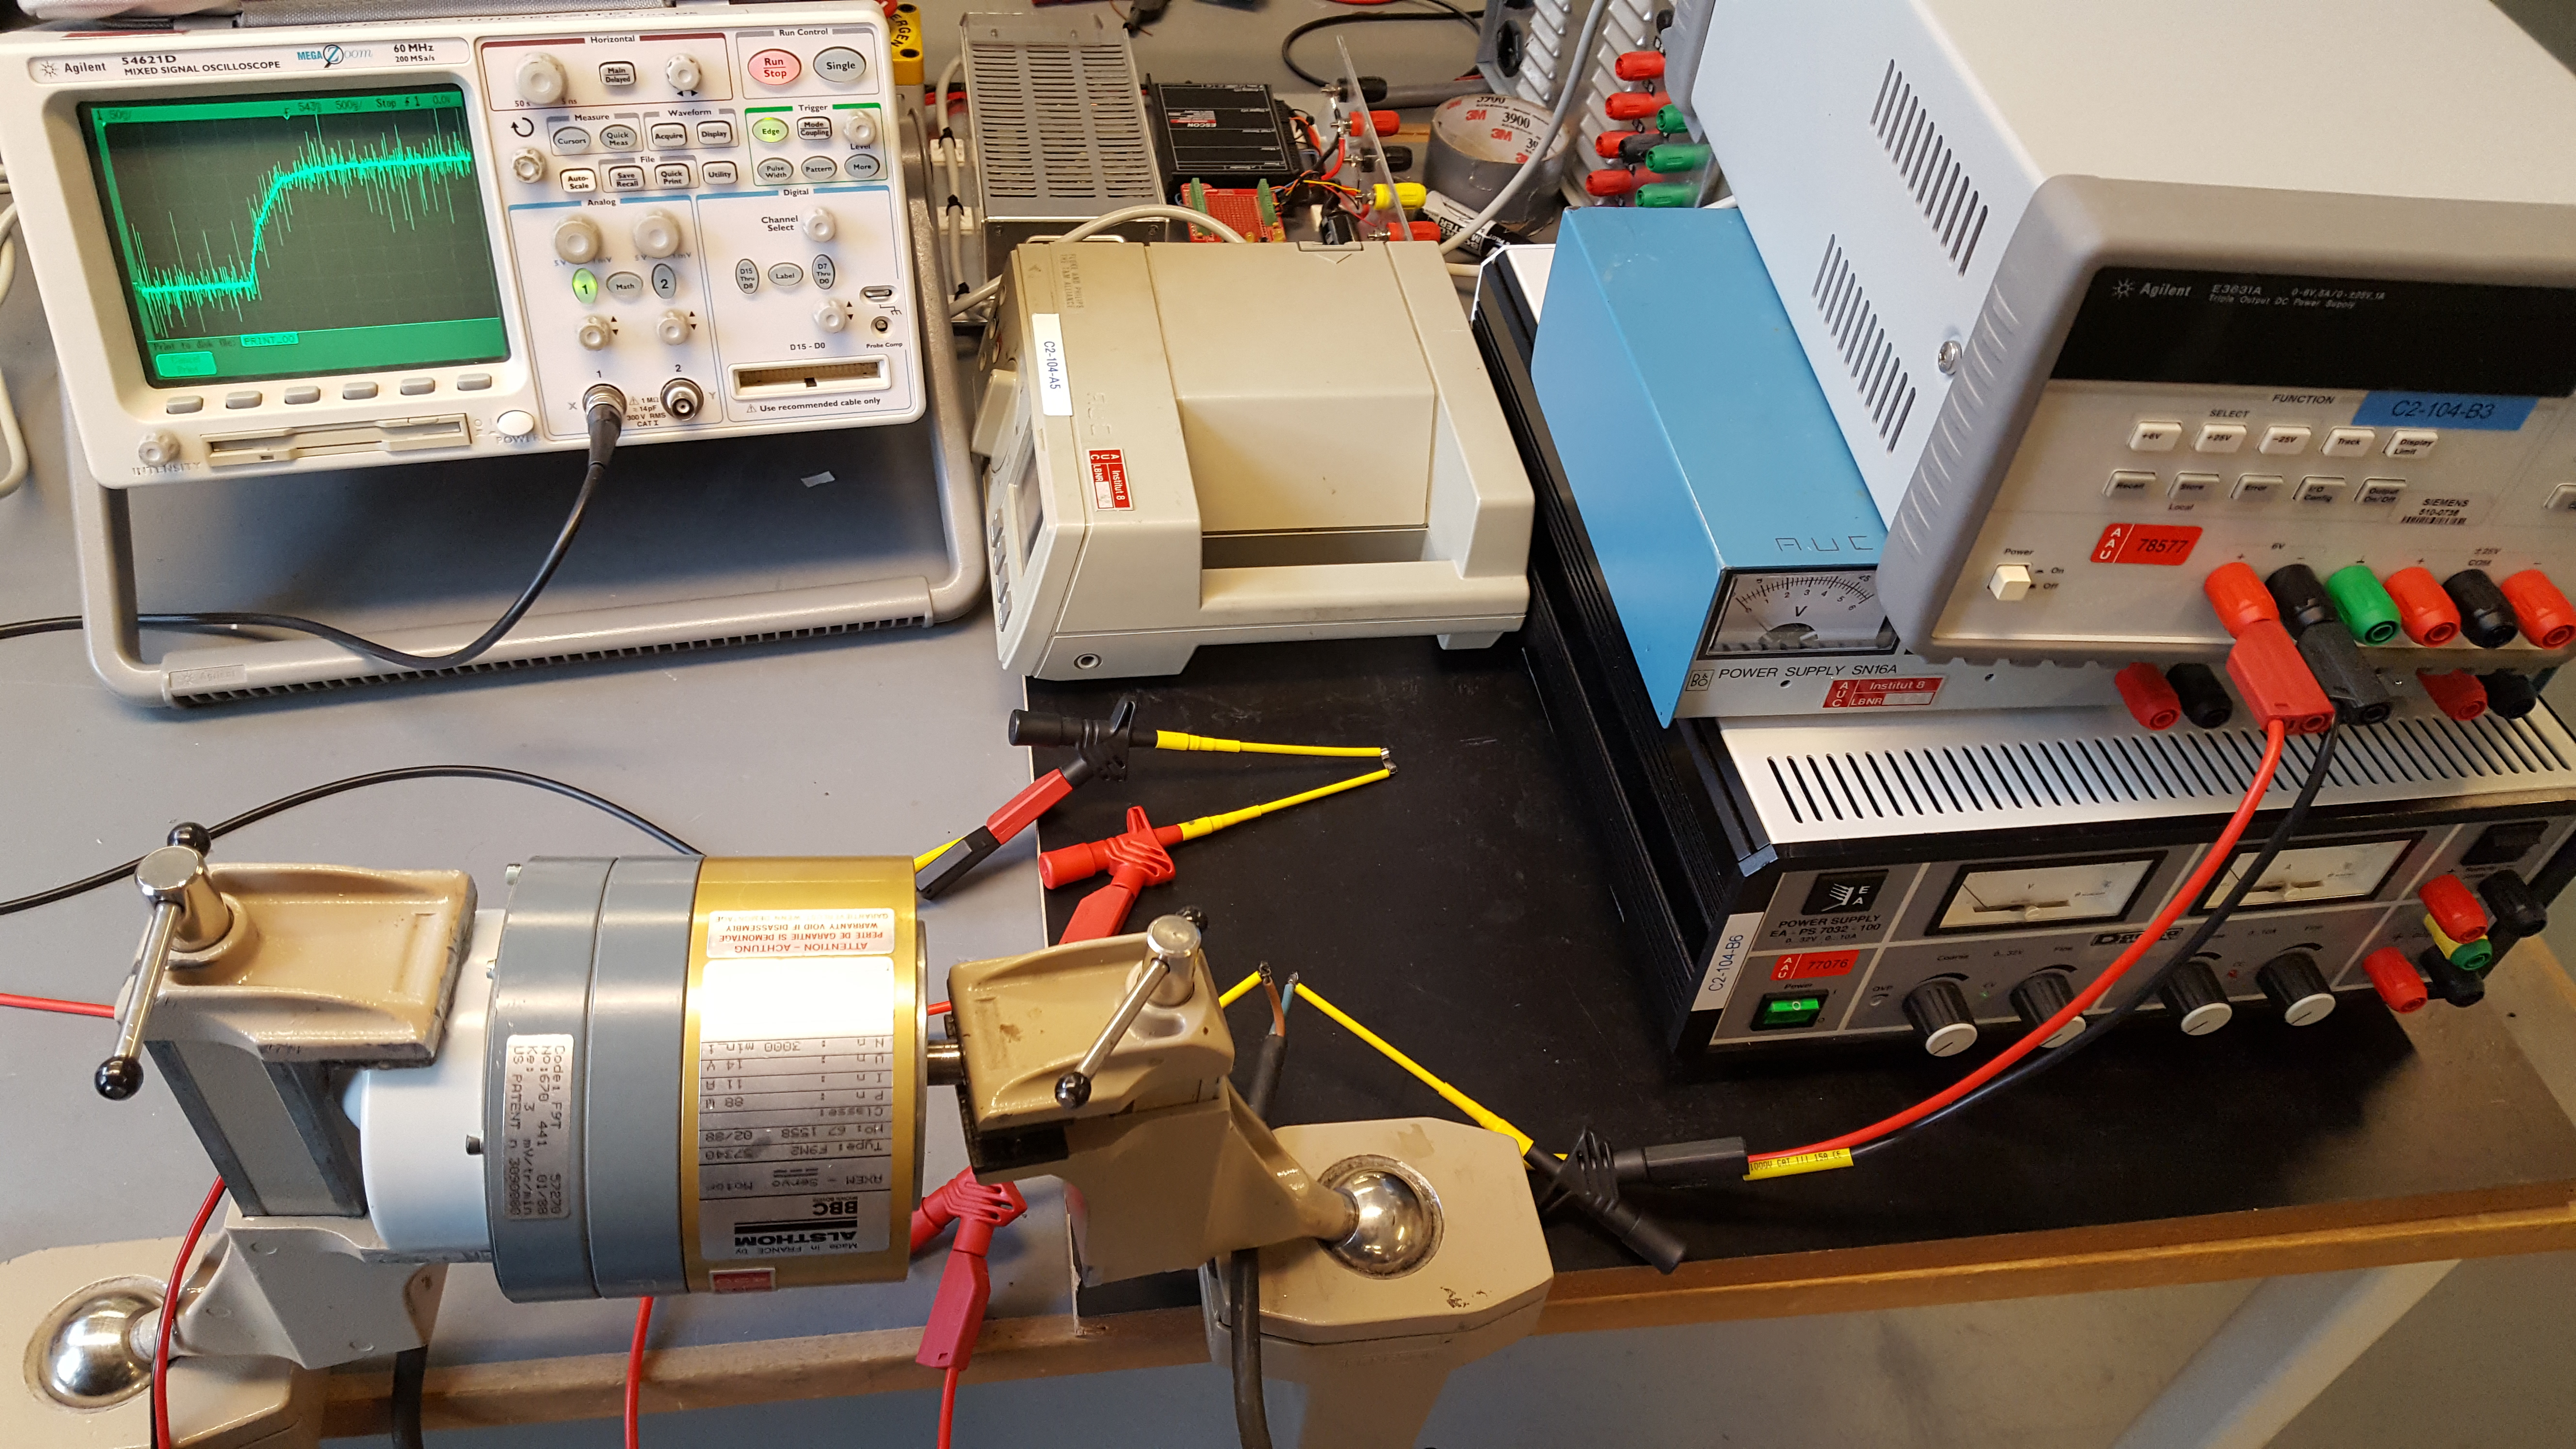
\includegraphics[width=1\textwidth]{MotorImpedanceTest.jpg}
		\missingfigure{Picture of the setup}
		\caption{Picture of the setup.} \label{fig:BmMeasurementPictures}
	\end{subfigure}
	\caption{The measurement set up.} \label{fig:BmMeasurementSetup}   
\end{figure}

\subsubsection*{Method}
This test consists of having the motor shaft running in steady state while the torque $\tau_m$, the shaft angular velocity $\omega$ and the current $I$ are measured.

\subsubsection*{Raw data}
\autoref{tab:KtTest} has all the measurements done.


\subsubsection*{Data processing}

The motor and the shaft are in steady state so $\tau_m=\tau_{fm}$ which combined with \autoref{eq:FrictionTorque} gives \autoref{eq:BmTest}.

\begin{equation}\label{eq:BmTest}
B_m=\frac{K_t I}{\omega} \addunit{\newton\per\radian\second}
\end{equation}
\startexplain
\explain{$I$ is the current in the circuit}{\si{\ampere}}
\explain{$K_t$ is the motor's torque constant}{\si{\newton\meter}}
\explain{$\omega$ is the shaft's angular velocity}{\si{\radian\per\second}}
\explain{$B_m$ is the viscous friction constant}{\si{\newton\per\radian\second}}
\stopexplain

\subsubsection*{Conclusion}

\autoref{fig:BmTest} plot the $B_m$ found for each measurement. The $B_m$ used in the model is average of these points. This gives $B_m=\SI{120}{\micro\newton\per\radian\second}$

\begin{figure}[htbp]
	\centering
	\includegraphics[width=\textwidth]{figures/appendix/Motor&GearTests/RmLmDataPlot}
	\caption{Plot of $B_m$ found for each measures}\label{fig:BmTest}
\end{figure}
\break

\subsection{Moment of Inertia $J_a$}
